\section{Toaster Design Case Study}

This section contains a simplistic case study of how the proposed algorithm could be used to compare the functional
requirement (FR) graphs resulting from two slightly different designs of the basic kitchen toaster shown in
Figure \ref{fig:toaster}.

\begin{figure}[h]
  \label{fig:toaster}
  \begin{center}
    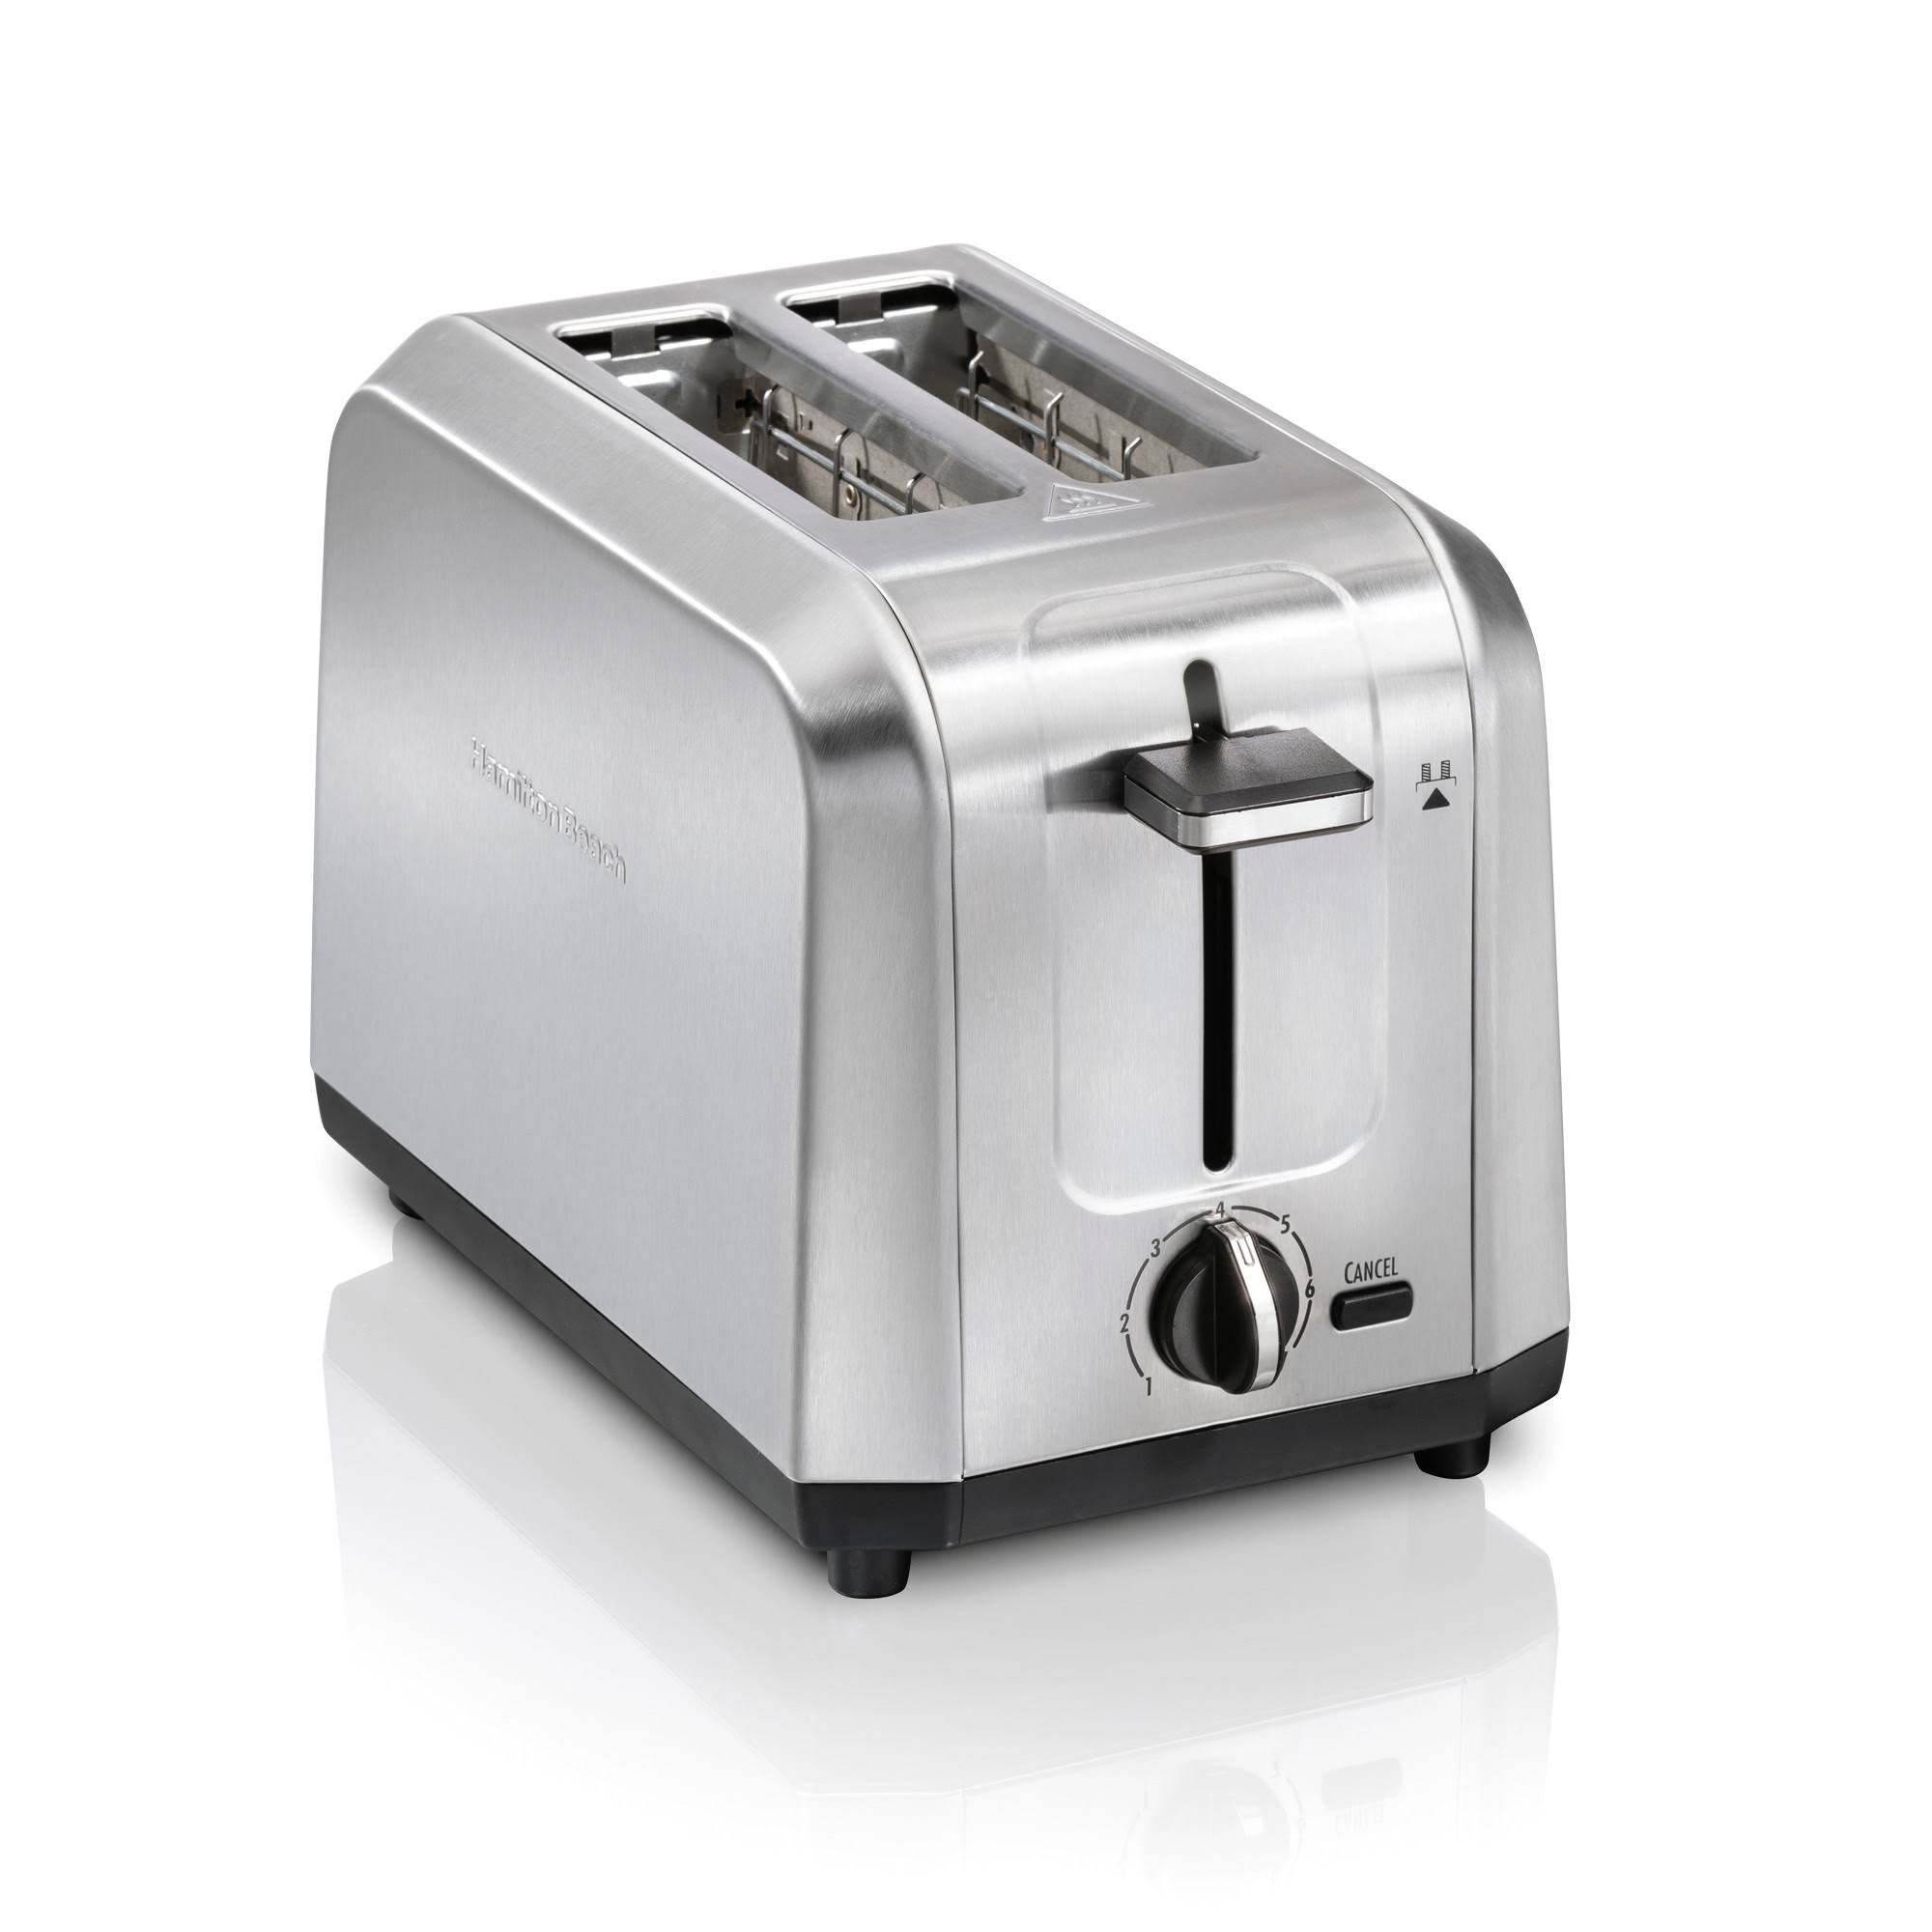
\includegraphics[scale=0.2]{toaster}
  \end{center}
  \caption{Example Toaster}
\end{figure}

The functional requirements (FRs) are shown in Table \ref{toasterfrs}.  It is assumed that the design is either
uncoupled or decoupled and hence the independence of the FRs is as strong as possible.

\begin{table}[h]
  \label{toasterfrs}
  \begin{center}
    \begin{tabular}{|c|l|}
      \hline
      FR1 & Body contains all parts \\
      \hline
      FR2 & Can be safely moved while hot \\
      \hline
      FR3 & Can hold two slices of bread \\
      \hline
      FR4 & Heats each slice of bread on both sides \\
      \hline
      FR5 & Toasting is manually started \\
      \hline
      FR6 & Toasting is automatically or can be manually stopped \\
      \hline
      FR7 & Heat level can be controlled \\
      \hline
    \end{tabular}
  \end{center}
  \caption{Toaster Functional Requirements}
\end{table}

The graph \(G_1\) for the first candidate design with \(n=7\) and \(m=13\) is shown in Figure \ref{fig:design1}.

\begin{figure}[h]
  \label{fig:design1}
  \begin{center}
    \scalebox{0.75}{
      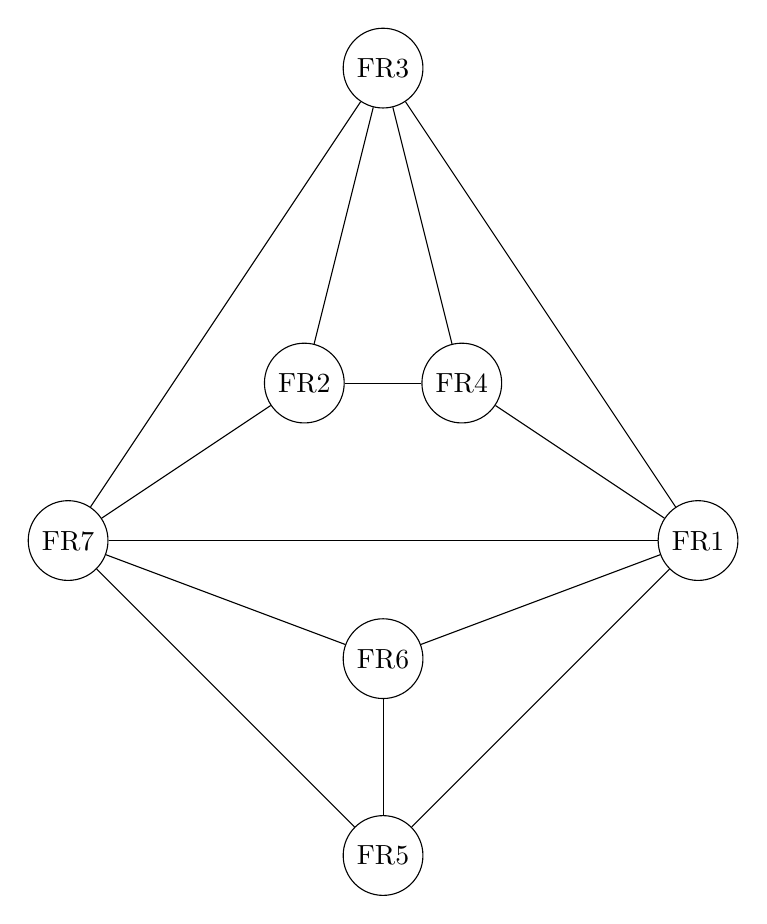
\begin{tikzpicture}
        \node [draw,circle] (fr1) at (4,0) {FR1};
        \node [draw,circle] (fr2) at (-1,2) {FR2};
        \node [draw,circle] (fr3) at (0,6) {FR3};
        \node [draw,circle] (fr4) at (1,2) {FR4};
        \node [draw,circle] (fr5) at (0,-4) {FR5};
        \node [draw,circle] (fr6) at (0,-1.5) {FR6};
        \node [draw,circle] (fr7) at (-4,0) {FR7};
        \draw (fr1) edge (fr3);
        \draw (fr1) edge (fr4);
        \draw (fr1) edge (fr5);
        \draw (fr1) edge (fr6);
        \draw (fr1) edge (fr7);
        \draw (fr2) edge (fr3);
        \draw (fr2) edge (fr4);
        \draw (fr2) edge (fr7);
        \draw (fr3) edge (fr4);
        \draw (fr3) edge (fr7);
        \draw (fr5) edge (fr6);
        \draw (fr5) edge (fr7);
        \draw (fr6) edge (fr7);
      \end{tikzpicture}
    }

    \bigskip

    \(G_1\)
  \end{center}
  \caption{First Candidate Design}
\end{figure}

For \(k=2\), the maximum edge threshold test fails:
\[\frac{n^2(k-1)}{2k}=\frac{7^2(2-1)}{2\cdot2}=\frac{49}{4}\approx12.3<13=m\]
so \(G_1\) is not \colorable{2}.

For \(k=3\), the maximum edge threshold test passes:
\[\frac{n^2(k-1)}{2k}=\frac{7^2(3-1)}{2\cdot3}=\frac{98}{6}\approx16.3>13=m\]
There are no vertices with degrees less than \(k=3\); however, note that \(N(\text{FR2})\subseteq N(\text{FR1})\),
so remove vertex FR2.  The result is shown in Figure \ref{fig:d1rem2}.

\begin{figure}[h]
  \label{fig:d1rem2}
  \begin{center}
    \scalebox{0.75}{
      \begin{tikzpicture}
        \node [draw,circle] (fr1) at (4,0) {FR1};
        \node [draw,circle] (fr3) at (0,6) {FR3};
        \node [draw,circle] (fr4) at (1,2) {FR4};
        \node [draw,circle] (fr5) at (0,-4) {FR5};
        \node [draw,circle] (fr6) at (0,-1.5) {FR6};
        \node [draw,circle] (fr7) at (-4,0) {FR7};
        \draw (fr1) edge (fr3);
        \draw (fr1) edge (fr4);
        \draw (fr1) edge (fr5);
        \draw (fr1) edge (fr6);
        \draw (fr1) edge (fr7);
        \draw (fr3) edge (fr4);
        \draw (fr3) edge (fr7);
        \draw (fr5) edge (fr6);
        \draw (fr5) edge (fr7);
        \draw (fr6) edge (fr7);
      \end{tikzpicture}
    }

    \bigskip

    \(G_1-\text{FR2}\)
  \end{center}
  \caption{Design 1---Remove FR2}
\end{figure}

Next, since \(\deg(\text{FR4})=2<3=k\), remove FR4.  As a result of removing FR4, \(\deg(\text{FR3})=2<3=k\), so
remove FR3 as well.  The result is show in Figure \ref{fig:d1rem34}.

\begin{figure}[h]
  \label{fig:d1rem34}
  \begin{center}
    \scalebox{0.75}{
      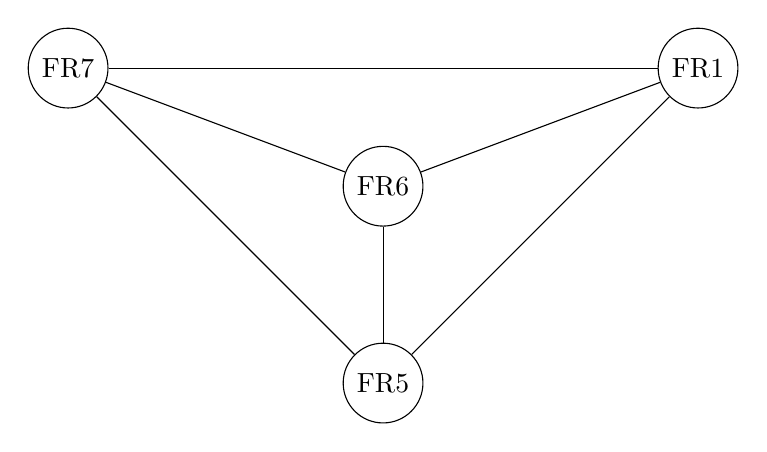
\begin{tikzpicture}
        \node [draw,circle] (fr1) at (4,0) {FR1};
        \node [draw,circle] (fr5) at (0,-4) {FR5};
        \node [draw,circle] (fr6) at (0,-1.5) {FR6};
        \node [draw,circle] (fr7) at (-4,0) {FR7};
        \draw (fr1) edge (fr5);
        \draw (fr1) edge (fr6);
        \draw (fr1) edge (fr7);
        \draw (fr5) edge (fr6);
        \draw (fr5) edge (fr7);
        \draw (fr6) edge (fr7);
      \end{tikzpicture}
    }

    \bigskip

    \(G_1-\text{FR4}-\text{FR3}\)
  \end{center}
  \caption{Design 1---Remove FR4 and FR3}
\end{figure}

At this point, \(G_1=K_4\), so it is guaranteed to fail the maximum edge threshold check for \(k=3\) and thus not
be \colorable{3}.  At \(k=4\) we have \(n=4\le4=k\).  Thus, we can conclude that \(G_1\) is \chromatic{4}. An
example chromatic coloring with:
\[C=\set{\text{\textcolor{green}{green}},\text{\textcolor{blue}{blue}},\text{\textcolor{red}{red}},
  \text{\textcolor{yellow}{yellow}}}\]
is show in Figure \ref{fig:d1color}.

\begin{figure}[h]
  \label{fig:d1color}
  \begin{center}
    \scalebox{0.75}{
      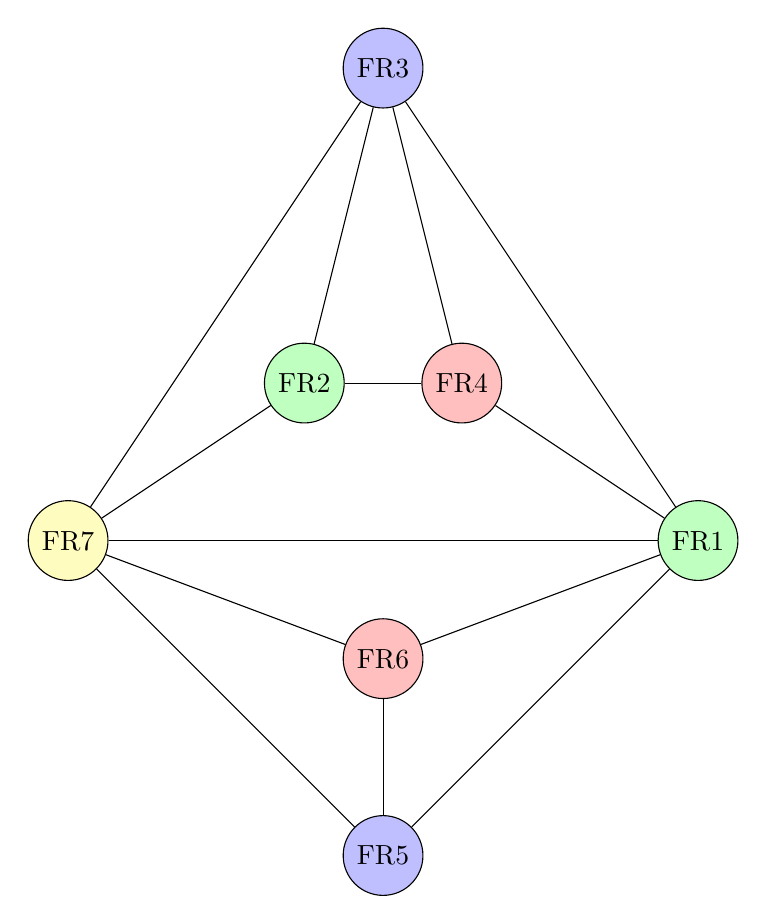
\begin{tikzpicture}
        \colorlet{c1}{green!25!white}
        \colorlet{c2}{blue!25!white}
        \colorlet{c3}{red!25!white}
        \colorlet{c4}{yellow!25!white}
        \node [draw,circle,fill=c1] (fr1) at (4,0) {FR1};
        \node [draw,circle,fill=c1] (fr2) at (-1,2) {FR2};
        \node [draw,circle,fill=c2] (fr3) at (0,6) {FR3};
        \node [draw,circle,fill=c3] (fr4) at (1,2) {FR4};
        \node [draw,circle,fill=c2] (fr5) at (0,-4) {FR5};
        \node [draw,circle,fill=c3] (fr6) at (0,-1.5) {FR6};
        \node [draw,circle,fill=c4] (fr7) at (-4,0) {FR7};
        \draw (fr1) edge (fr3);
        \draw (fr1) edge (fr4);
        \draw (fr1) edge (fr5);
        \draw (fr1) edge (fr6);
        \draw (fr1) edge (fr7);
        \draw (fr2) edge (fr3);
        \draw (fr2) edge (fr4);
        \draw (fr2) edge (fr7);
        \draw (fr3) edge (fr4);
        \draw (fr3) edge (fr7);
        \draw (fr5) edge (fr6);
        \draw (fr5) edge (fr7);
        \draw (fr6) edge (fr7);
      \end{tikzpicture}
    }

    \bigskip

    \(G_1\)
  \end{center}
  \caption{Design 1---Chromatic Coloring}
\end{figure}

Notice in the design that FR5 (start toasting) and FR6 (stop toasting) have been forced into separate parts,
conceivably to accommodate the separate ``cancel'' button shown in Figure \ref{fig:toaster}.  But what if the
designer decides to eliminate the cancel button and allow manual cancellation via the lever?  Thus, FR5 and FR6
no longer need to be separated, so the edge between their vertices can be eliminated.  The result is shown in Figure
\ref{fig:design2}.

\begin{figure}[h]
  \label{fig:design2}
  \begin{center}
    \scalebox{0.75}{
      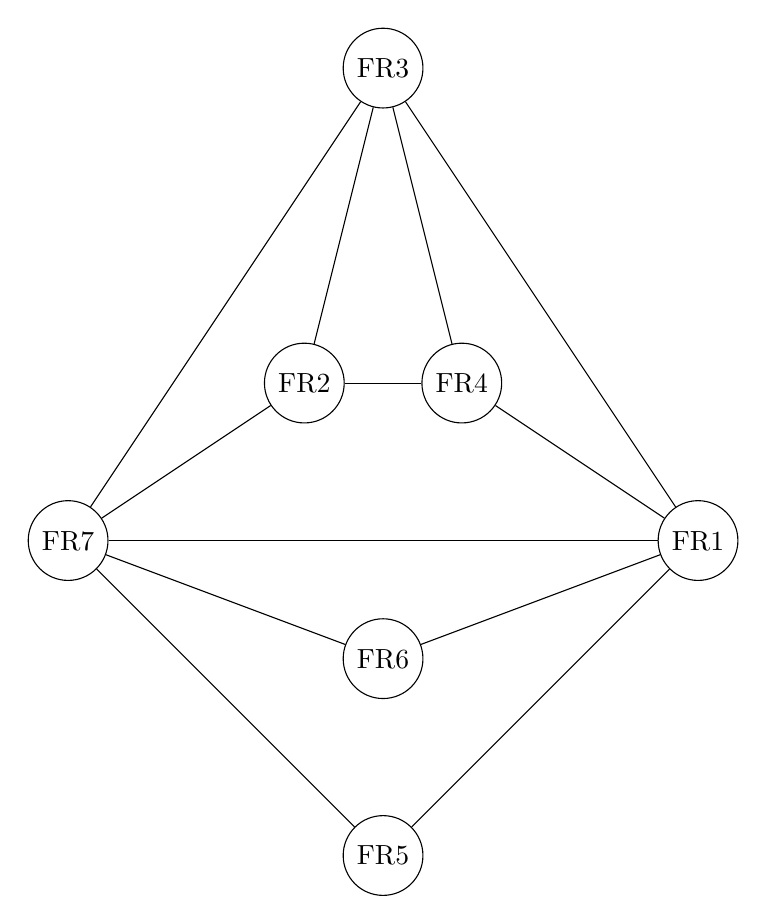
\begin{tikzpicture}
        \node [draw,circle] (fr1) at (4,0) {FR1};
        \node [draw,circle] (fr2) at (-1,2) {FR2};
        \node [draw,circle] (fr3) at (0,6) {FR3};
        \node [draw,circle] (fr4) at (1,2) {FR4};
        \node [draw,circle] (fr5) at (0,-4) {FR5};
        \node [draw,circle] (fr6) at (0,-1.5) {FR6};
        \node [draw,circle] (fr7) at (-4,0) {FR7};
        \draw (fr1) edge (fr3);
        \draw (fr1) edge (fr4);
        \draw (fr1) edge (fr5);
        \draw (fr1) edge (fr6);
        \draw (fr1) edge (fr7);
        \draw (fr2) edge (fr3);
        \draw (fr2) edge (fr4);
        \draw (fr2) edge (fr7);
        \draw (fr3) edge (fr4);
        \draw (fr3) edge (fr7);
        \draw (fr5) edge (fr7);
        \draw (fr6) edge (fr7);
      \end{tikzpicture}
    }

    \bigskip

    \(G_2\)
  \end{center}
  \caption{Second Candidate Design}
\end{figure}

Rerun the algorithm on \(G_2\) for \(n=7\) and \(m=12\).  For \(k=2\), the maximum edge threshold test passes:
\[\frac{n^2(k-1)}{2k}=\frac{7^2(2-1)}{2\cdot2}=\frac{49}{4}\approx12.3>12=m\]
Note that \(N(\text{FR6})\subseteq N(\text{FR5})\), so remove FR6.  The result is shown in Figure \ref{fig:d2rem6}.

\begin{figure}[h]
  \label{fig:d2rem6}
  \begin{center}
    \scalebox{0.75}{
      \begin{tikzpicture}
        \node [draw,circle] (fr1) at (4,0) {FR1};
        \node [draw,circle] (fr2) at (-1,2) {FR2};
        \node [draw,circle] (fr3) at (0,6) {FR3};
        \node [draw,circle] (fr4) at (1,2) {FR4};
        \node [draw,circle] (fr5) at (0,-4) {FR5};
        \node [draw,circle] (fr7) at (-4,0) {FR7};
        \draw (fr1) edge (fr3);
        \draw (fr1) edge (fr4);
        \draw (fr1) edge (fr5);
        \draw (fr1) edge (fr7);
        \draw (fr2) edge (fr3);
        \draw (fr2) edge (fr4);
        \draw (fr2) edge (fr7);
        \draw (fr3) edge (fr4);
        \draw (fr3) edge (fr7);
        \draw (fr5) edge (fr7);
      \end{tikzpicture}
    }

    \bigskip

    \(G_2-\text{FR6}\)
  \end{center}
  \caption{Design 2---Remove FR6}
\end{figure}

Now, with \(n=6\) and \(m=10\), \(G_2\) fails the maximum edge threshold test for \(k=2\):
\[\frac{n^2(k-1)}{2k}=\frac{6^2(2-1)}{2\cdot2}=\frac{36}{4}=9<10=m\]
so \(G_2\) is not \colorable{2}.

For \(k=3\), note that \(\deg(\text{FR5})=2<3=k\), so remove FR5.  The result is shown in Figure \ref{fig:d2rem5}.

\begin{figure}[h]
  \label{fig:d2rem5}
  \begin{center}
    \scalebox{0.75}{
      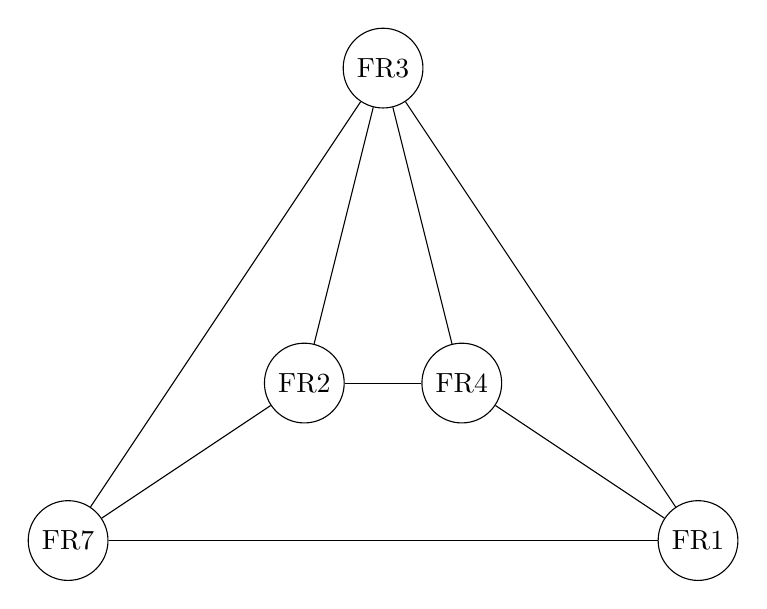
\begin{tikzpicture}
        \node [draw,circle] (fr1) at (4,0) {FR1};
        \node [draw,circle] (fr2) at (-1,2) {FR2};
        \node [draw,circle] (fr3) at (0,6) {FR3};
        \node [draw,circle] (fr4) at (1,2) {FR4};
        \node [draw,circle] (fr7) at (-4,0) {FR7};
        \draw (fr1) edge (fr3);
        \draw (fr1) edge (fr4);
        \draw (fr1) edge (fr7);
        \draw (fr2) edge (fr3);
        \draw (fr2) edge (fr4);
        \draw (fr2) edge (fr7);
        \draw (fr3) edge (fr4);
        \draw (fr3) edge (fr7);
      \end{tikzpicture}
    }

    \bigskip

    \(G_2-\text{FR5}\)
  \end{center}
  \caption{Design 2---Remove FR5}
\end{figure}

Now, with \(n=5\) and \(m=8\), \(G_2\) passes the maximum edge threshold test for \(k=3\):
\[\frac{n^2(k-1)}{2k}=\frac{5^2(3-1)}{2\cdot3}=\frac{50}{6}\approx8.3>8=m\]
Since \(N(\text{FR2})\subseteq N(\text{FR1})\), remove FR2.  The result is shown in Figure \ref{fig:d2rem2}.

\begin{figure}[h]
  \label{fig:d2rem2}
  \begin{center}
    \scalebox{0.75}{
      \begin{tikzpicture}
        \node [draw,circle] (fr1) at (4,0) {FR1};
        \node [draw,circle] (fr3) at (0,6) {FR3};
        \node [draw,circle] (fr4) at (1,2) {FR4};
        \node [draw,circle] (fr7) at (-4,0) {FR7};
        \draw (fr1) edge (fr3);
        \draw (fr1) edge (fr4);
        \draw (fr1) edge (fr7);
        \draw (fr3) edge (fr4);
        \draw (fr3) edge (fr7);
      \end{tikzpicture}
    }

    \bigskip

    \(G_2-\text{FR2}\)
  \end{center}
  \caption{Design 2---Remove FR2}
\end{figure}

Finally, \(\deg(\text{FR4})=\deg(\text{FR7})=2<3=k\), so remove FR4 and FR7.  The result is shown in Figure
\ref{fig:d2rem47}.

\begin{figure}[h]
  \label{fig:d2rem47}
  \begin{center}
    \scalebox{0.75}{
      \begin{tikzpicture}
        \node [draw,circle] (fr1) at (4,0) {FR1};
        \node [draw,circle] (fr3) at (0,6) {FR3};
        \draw (fr1) edge (fr3);
      \end{tikzpicture}
    }

    \bigskip

    \(G_2-\text{FR4,FR7}\)
  \end{center}
  \caption{Design 2---Remove FR4 and FR7}
\end{figure}

This final state of \(G_2\) has \(n=2\le3=k\), so we can conclude that \(G_2\) is \chromatic{3}.  An example
chromatic coloring with:
\[C=\set{\text{\textcolor{green}{green}},\text{\textcolor{blue}{blue}},\text{\textcolor{red}{red}}}\]
is show in Figure \ref{fig:d2color}.
\begin{figure}[h]
  \label{fig:d2color}
  \begin{center}
    \scalebox{0.75}{
      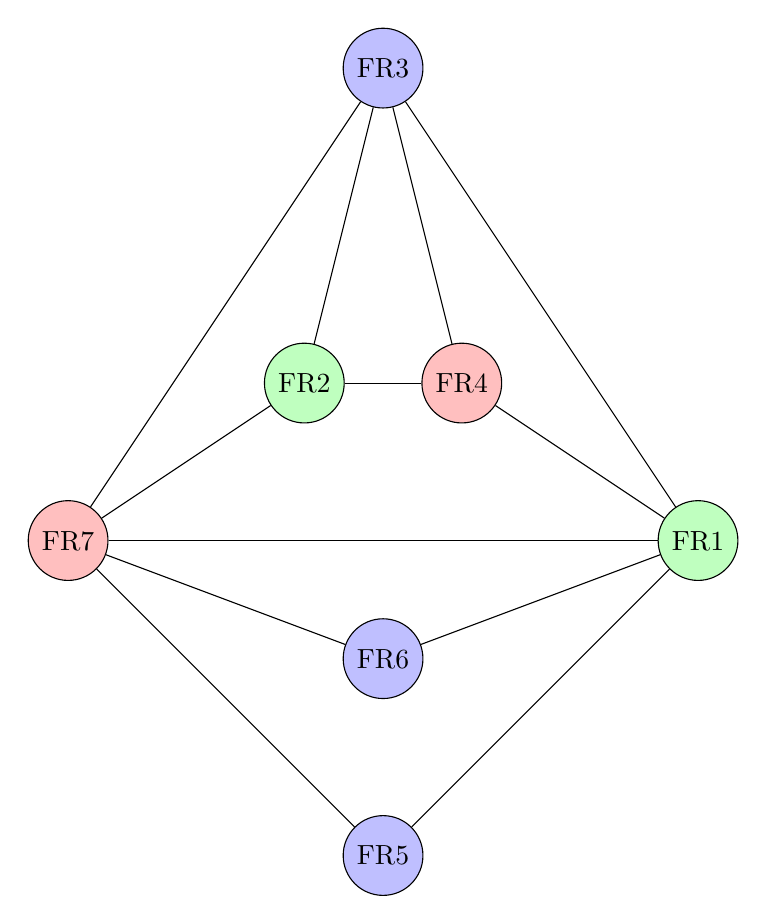
\begin{tikzpicture}
        \colorlet{c1}{green!25!white}
        \colorlet{c2}{blue!25!white}
        \colorlet{c3}{red!25!white}
        \node [draw,circle,fill=c1] (fr1) at (4,0) {FR1};
        \node [draw,circle,fill=c1] (fr2) at (-1,2) {FR2};
        \node [draw,circle,fill=c2] (fr3) at (0,6) {FR3};
        \node [draw,circle,fill=c3] (fr4) at (1,2) {FR4};
        \node [draw,circle,fill=c2] (fr5) at (0,-4) {FR5};
        \node [draw,circle,fill=c2] (fr6) at (0,-1.5) {FR6};
        \node [draw,circle,fill=c3] (fr7) at (-4,0) {FR7};
        \draw (fr1) edge (fr3);
        \draw (fr1) edge (fr4);
        \draw (fr1) edge (fr5);
        \draw (fr1) edge (fr6);
        \draw (fr1) edge (fr7);
        \draw (fr2) edge (fr3);
        \draw (fr2) edge (fr4);
        \draw (fr2) edge (fr7);
        \draw (fr3) edge (fr4);
        \draw (fr3) edge (fr7);
        \draw (fr5) edge (fr7);
        \draw (fr6) edge (fr7);
      \end{tikzpicture}
    }

    \bigskip

    \(G_2\)
  \end{center}
  \caption{Design 2---Chromatic Coloring}
\end{figure}

This process gives the designer the feedback that the second design requires only three parts instead of four, and
thus has less information content and hence a higher chance of success than the first design.  It will be up to the
designer to weigh this result against other aspects of the design.
